\chapter{考察}
\label{ch:discussion}
\ref{ch:discussion}章ではミリ波分光計を用いて得られた\ref{ch:results}章での結果と、ミリ波分光計以外の外部からのデータの比較とを行う。
\ref{sec:comparison_sofie}節では、ノルウェー・トロムソにおける解析結果(\ref{sec:results_tromsoe}節)において、SOFIE:(Solar Occultation for Ice Experiment。詳細は付録\ref{app:sofie})によって観測された\ce{NO}密度の高度プロファイルデータを用いて比較を行う。
\ref{sec:comparison_eep}節では、EPPの影響を調べるため、高エネルギー電子の降り込み(EEP: Energetic Electron Precipitation)との比較を行う。


\section{SOFIEデータによって導出されたNO柱密度との比較}
\label{sec:comparison_sofie}
まずは、ミリ波分光計を用いた\ce{NO}の観測データの妥当性を確認するため、SOFIEによる\ce{NO}の密度の高度プロファイルデータを用いた。
本研究では、トロムソの柱密度を導出した期間と同じ時期にトロムソ付近の緯度(およそ$65 - 80$\textdegree Nの範囲)で観測されたSOFIEのデータを用いた。
その比較結果を図\ref{fig:sofie_mmcd}に示す。
なお、昭和基地においては、解析を行った期間のSOFIE観測データが\today 時点で公開されていないため比較を行っていない。
\begin{figure}[htbp]
    \centering
    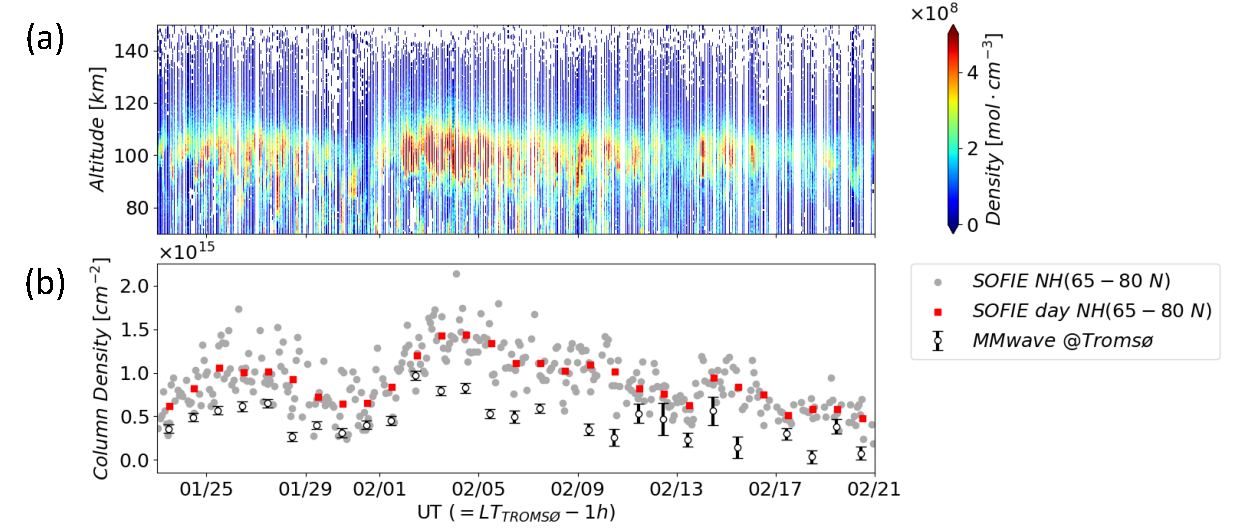
\includegraphics[width=\linewidth]{master_thesis_contents/master_thesis_fig/sofie_mmcd.pdf}
    \caption{(a)SOFIEの\ce{NO}密度の高度プロファイルデータおよび(b)ミリ波分光計を用いて導出したトロムソの柱密度とSOFIEの\ce{NO}密度の高度プロファイルデータから導出した柱密度の比較(エラーバー付きのプロットがミリ波データから導出した柱密度、グレーの丸形プロットがSOFIEの\ce{NO}密度の高度プロファイルデータから導出した柱密度、赤色の四角プロットが1日平均したSOFIEの柱密度)}
    \label{fig:sofie_mmcd}
\end{figure}
ミリ波分光計を用いて導出した柱密度の増加が確認された2つの時期(2019年1月23日〜2019年1月27日と2019年2月1日〜2019年2月4日)において、SOFIEの高度プロファイルデータでも高度$100\ \mathrm{km}$付近において\ce{NO}の密度の増加が確認できた(図\ref{fig:sofie_mmcd}(a))。
また、SOFIEの\ce{NO}密度の高度プロファイルデータを高度方向に足し合わせて、各高度プロファイルデータごとに柱密度を導出した(図\ref{fig:sofie_mmcd}(b)のグレーの丸形プロット)。
ミリ波分光計を用いて導出した柱密度との比較を行うため、SOFIEから導出した柱密度について1日平均した値を計算し、ミリ波分光計から導出した柱密度とのプロット間隔に合わせることで比較を行った。
その結果、ミリ波分光計による柱密度が、SOFIEから導出した柱密度と傾向が一致していることが分かった。
しかし、全体的にSOFIEから導出した柱密度が、ミリ波分光計による柱密度と比べて全体的に値が大きいことが分かった。
柱密度を導出する際に用いた式(\ref{sec:derive_columndensity}節の式\eqref{eq:derive_columndensity})より、第1項$A$と第2項$T_{\mathrm{atm}}$は観測条件によらない定数であり、第3項$\int T_{\mathrm{NO}}d\nu$のみが変数となるため、SOFIEから導出した柱密度とミリ波分光計による柱密度が定常倍であると仮定して比較を行った。
その結果を図\ref{fig:sofie_mmcd_sofiecd_corr}に示す。
\begin{figure}[htbp]
    \centering
    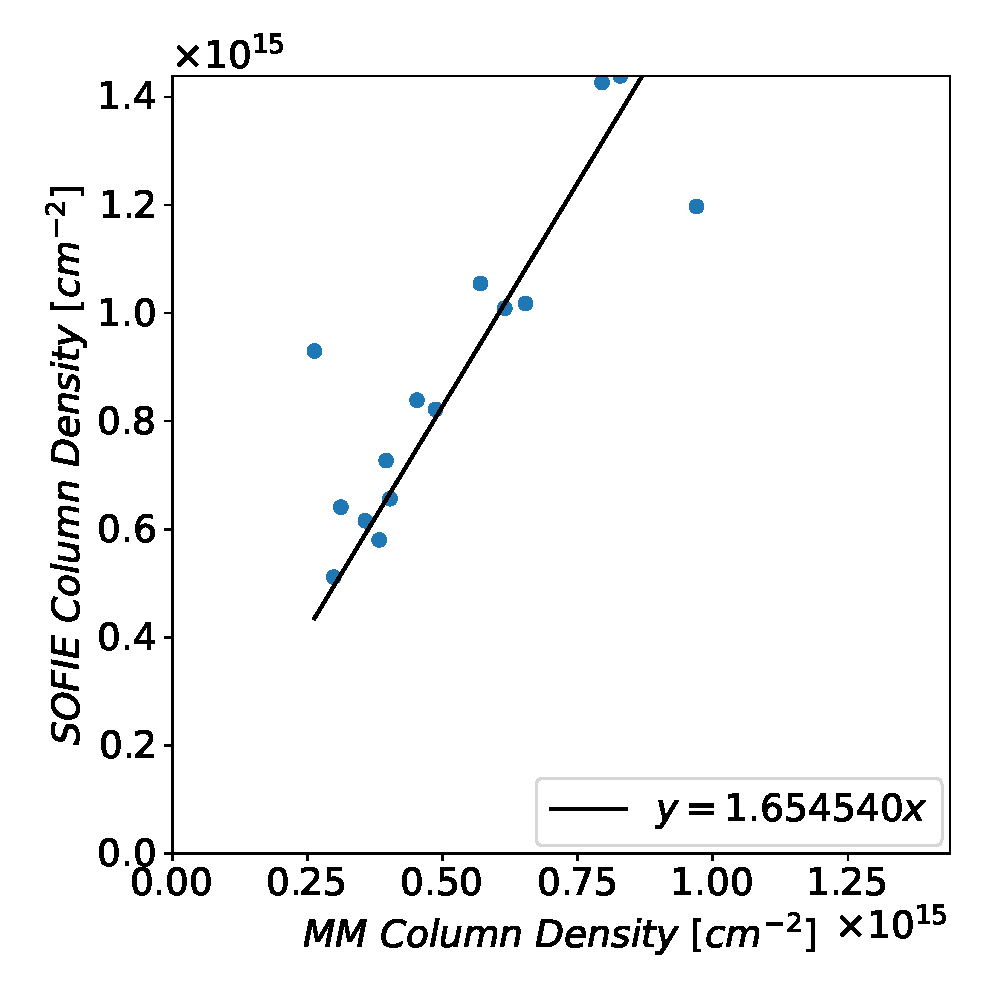
\includegraphics[scale=0.5]{master_thesis_contents/master_thesis_fig/sofie_mmcd_sofiecd_corr.pdf}
    \caption{ミリ波分光計から求めた柱密度(横軸)とSOFIEデータから求めた柱密度の1日平均値(縦軸)との散布図(青色のプロット。黒線は一次近似による直線を示し、右下はその式を表している)}
    \label{fig:sofie_mmcd_sofiecd_corr}
\end{figure}
ミリ波分光計から求めた柱密度とSOFIEデータから求めた柱密度の1日平均値について散布図をとった。
ただし、スクリーニングされた期間(2019年2月5日〜2019年2月16日)のプロットと、検知限界($2\times 10^{14}\ \mathrm{cm^{-2}}$)を下回るプロットは含めていない。
加えて、散布図上にあるプロットについて切片を0にした状態で一次近似を行った(図\ref{fig:sofie_mmcd_sofiecd_corr}の黒線。近似した直線の式は図の右下に示す)。
この結果より、SOFIEデータによって導出されたNO柱密度はミリ波分光計データによって導出された柱密度のおよそ1.65倍の大きさであることが分かった。
この原因の一部として、ミリ波分光計データによって柱密度を導出する際に仮定した大気温度(\ref{sec:derive_columndensity}節の式\eqref{eq:derive_columndensity}の第2項$T_{\mathrm{atm}}$)の値が妥当ではない可能性が考えられる。
そこで、NRLMSIS 2.0\footnote{\url{https://ccmc.gsfc.nasa.gov/models/NRLMSIS~00/}}を用いて、大気温度の妥当な値を調べた。
これを用いて、2019年1月25日と2月2日(ミリ波分光計を用いて導出した\ce{NO}の柱密度の時間変動のピーク)における高度$100\ \mathrm{km}$付近(SOFIEの\ce{NO}の密度の高度プロファイルデータにおける、ピークがある高度)の大気温度を調べたところ、およそ$180-250\ \mathrm{K}$の範囲であった。
仮に大気温度を$250\ \mathrm{K}$に仮定し直すと、ミリ波分光計を用いて導出した\ce{NO}の柱密度は1.25倍されるが、これだけではSOFIEで導出した\ce{NO}の柱密度との値の差を説明することはできない。
また、大気温度を高度に依存せず一様と仮定していることも原因として考えられるため、大気温度を高度ごとに設定することも考慮に入れる必要がある。


\section{高エネルギー電子の降り込みとの比較}
\label{sec:comparison_eep}
次に、EPPの影響を調べるため、高エネルギー電子の降り込みとの比較を行った。
比較対象として以下の3種類のデータを用い、各節に分けて比較結果を述べる。
\begin{itemize}
    \item Dst指数(\ref{ssec:comparison_dst}節)
    \item POES/MetOp衛星で観測された電子フラックスデータ(\ref{ssec:comparison_poes}節)
    \item NASAが提供しているOMNI Data Set(\ref{ssec:comparison_omni}節)
\end{itemize} \par
Dst指数、POES/MetOp、OMNI Data Setの詳細はそれぞれ付録\ref{app:dst}、付録\ref{app:poes}、付録\ref{app:omni}にて紹介している。


\subsection{Dst指数との比較}
\label{ssec:comparison_dst}
まずは、Dst指数との比較を行った。
Dst指数のデータは地磁気世界資料センター京都(WDC for Geomagnetism, Kyoto)\footnote{\url{https://wdc.kugi.kyoto-u.ac.jp/wdc/Sec3.html}}より調べた。
Dst指数とは、地磁気擾乱の大きさを表す指数であり、地磁気擾乱が起きる際に発生する、地球を取り巻く環状の電流(Ring Current)がどの程度地球磁場をどのくらい打ち消すかを表したものである(詳細は付録\ref{app:dst})。
トロムソにおける柱密度との比較結果を図\ref{fig:dst_mmcd_tromsoe}、昭和基地における柱密度との比較結果を図\ref{fig:dst_mmcd_syowa}に示す。
\begin{figure}[htbp]
    \centering
    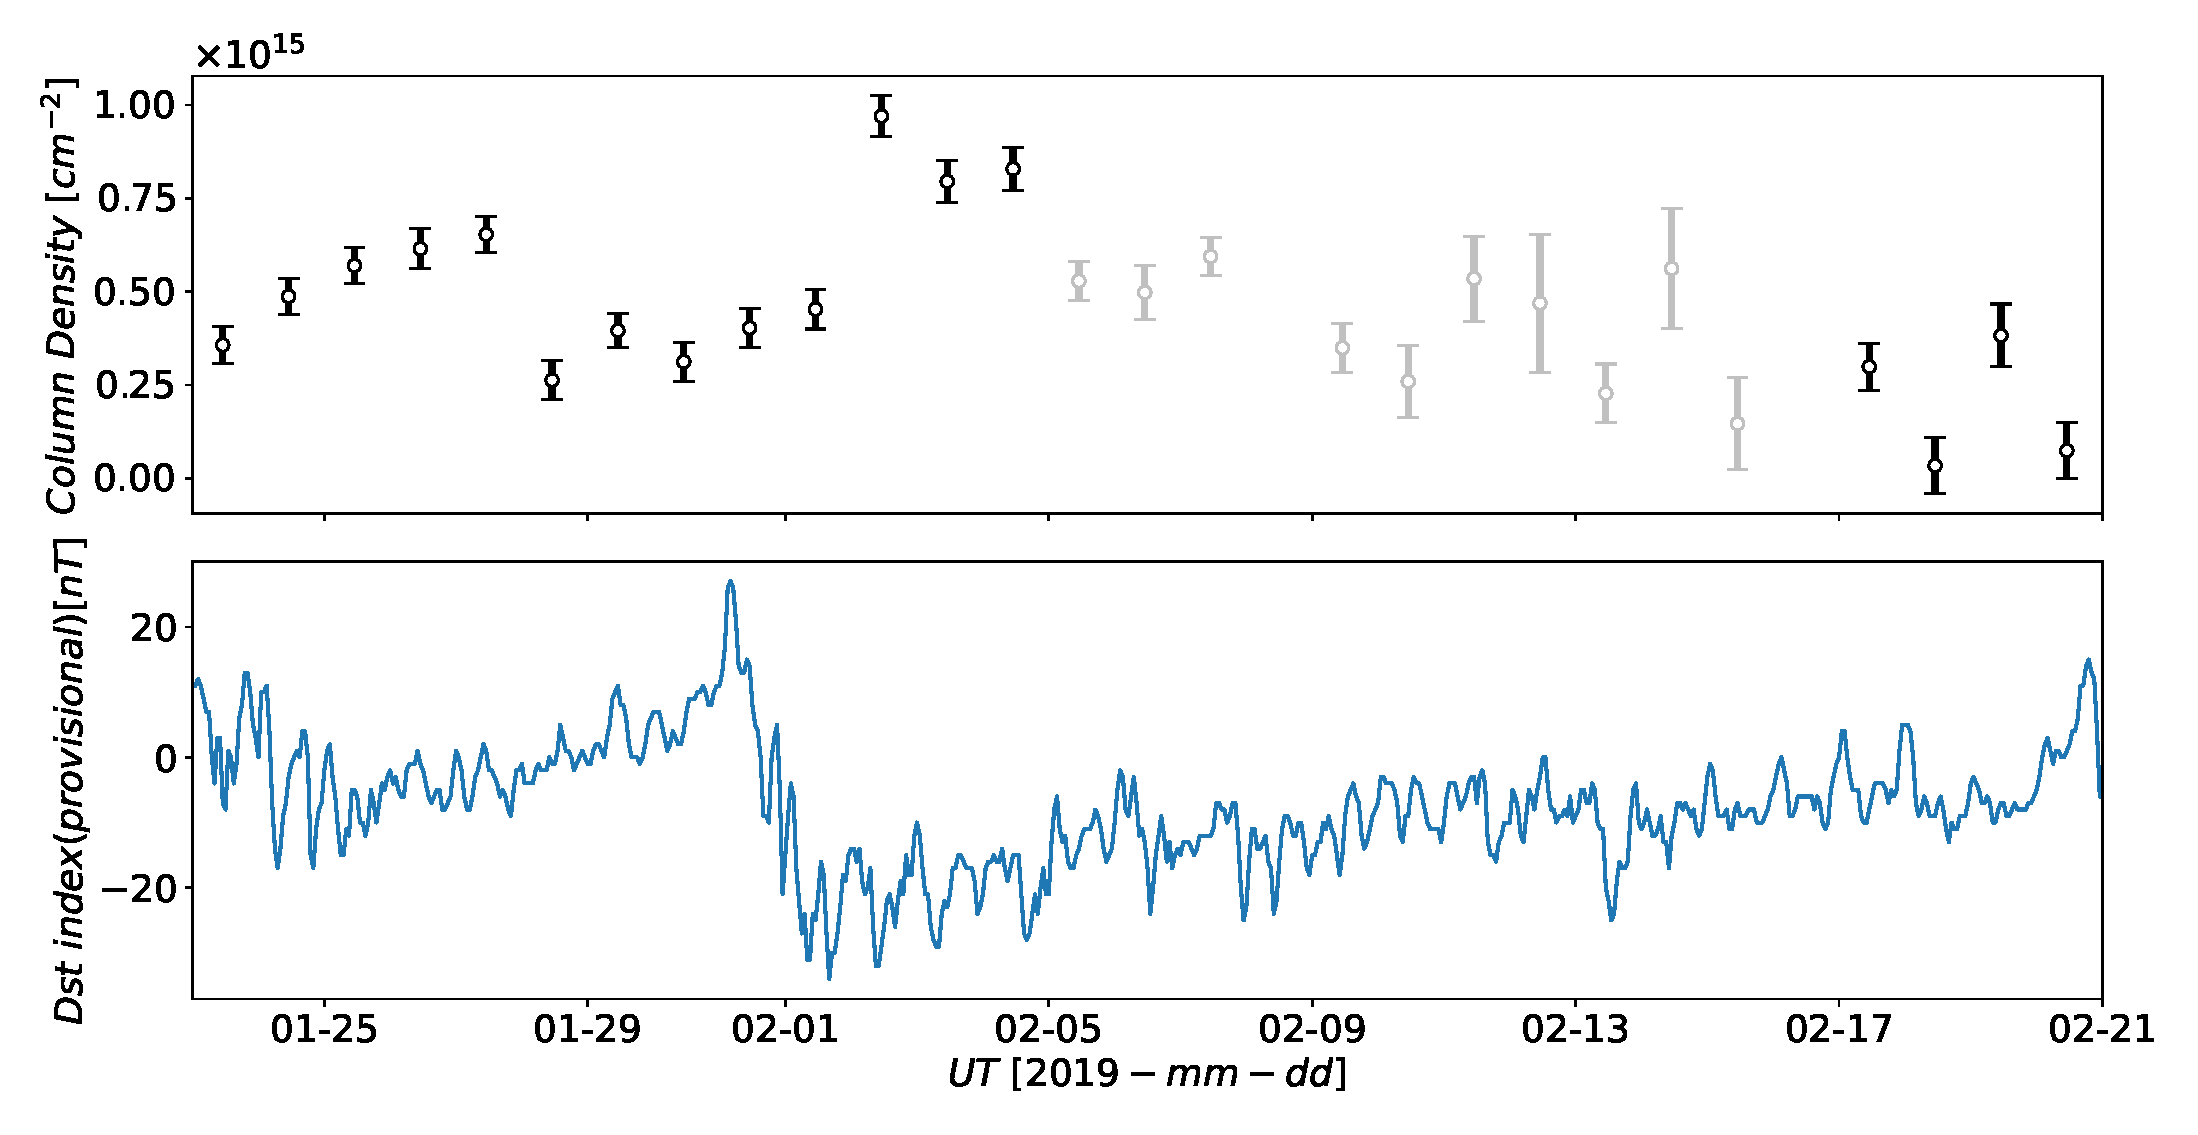
\includegraphics[width=\linewidth]{master_thesis_contents/master_thesis_fig/dst_tromsoe_mmcd.pdf}
    \caption{トロムソにおける柱密度(1段目。図\ref{fig:column_density_spectr6_syowa}と同様)とDst指数 暫定値(2段目)との比較}
    \label{fig:dst_mmcd_tromsoe}
\end{figure}
\begin{figure}[htbp]
    \centering
    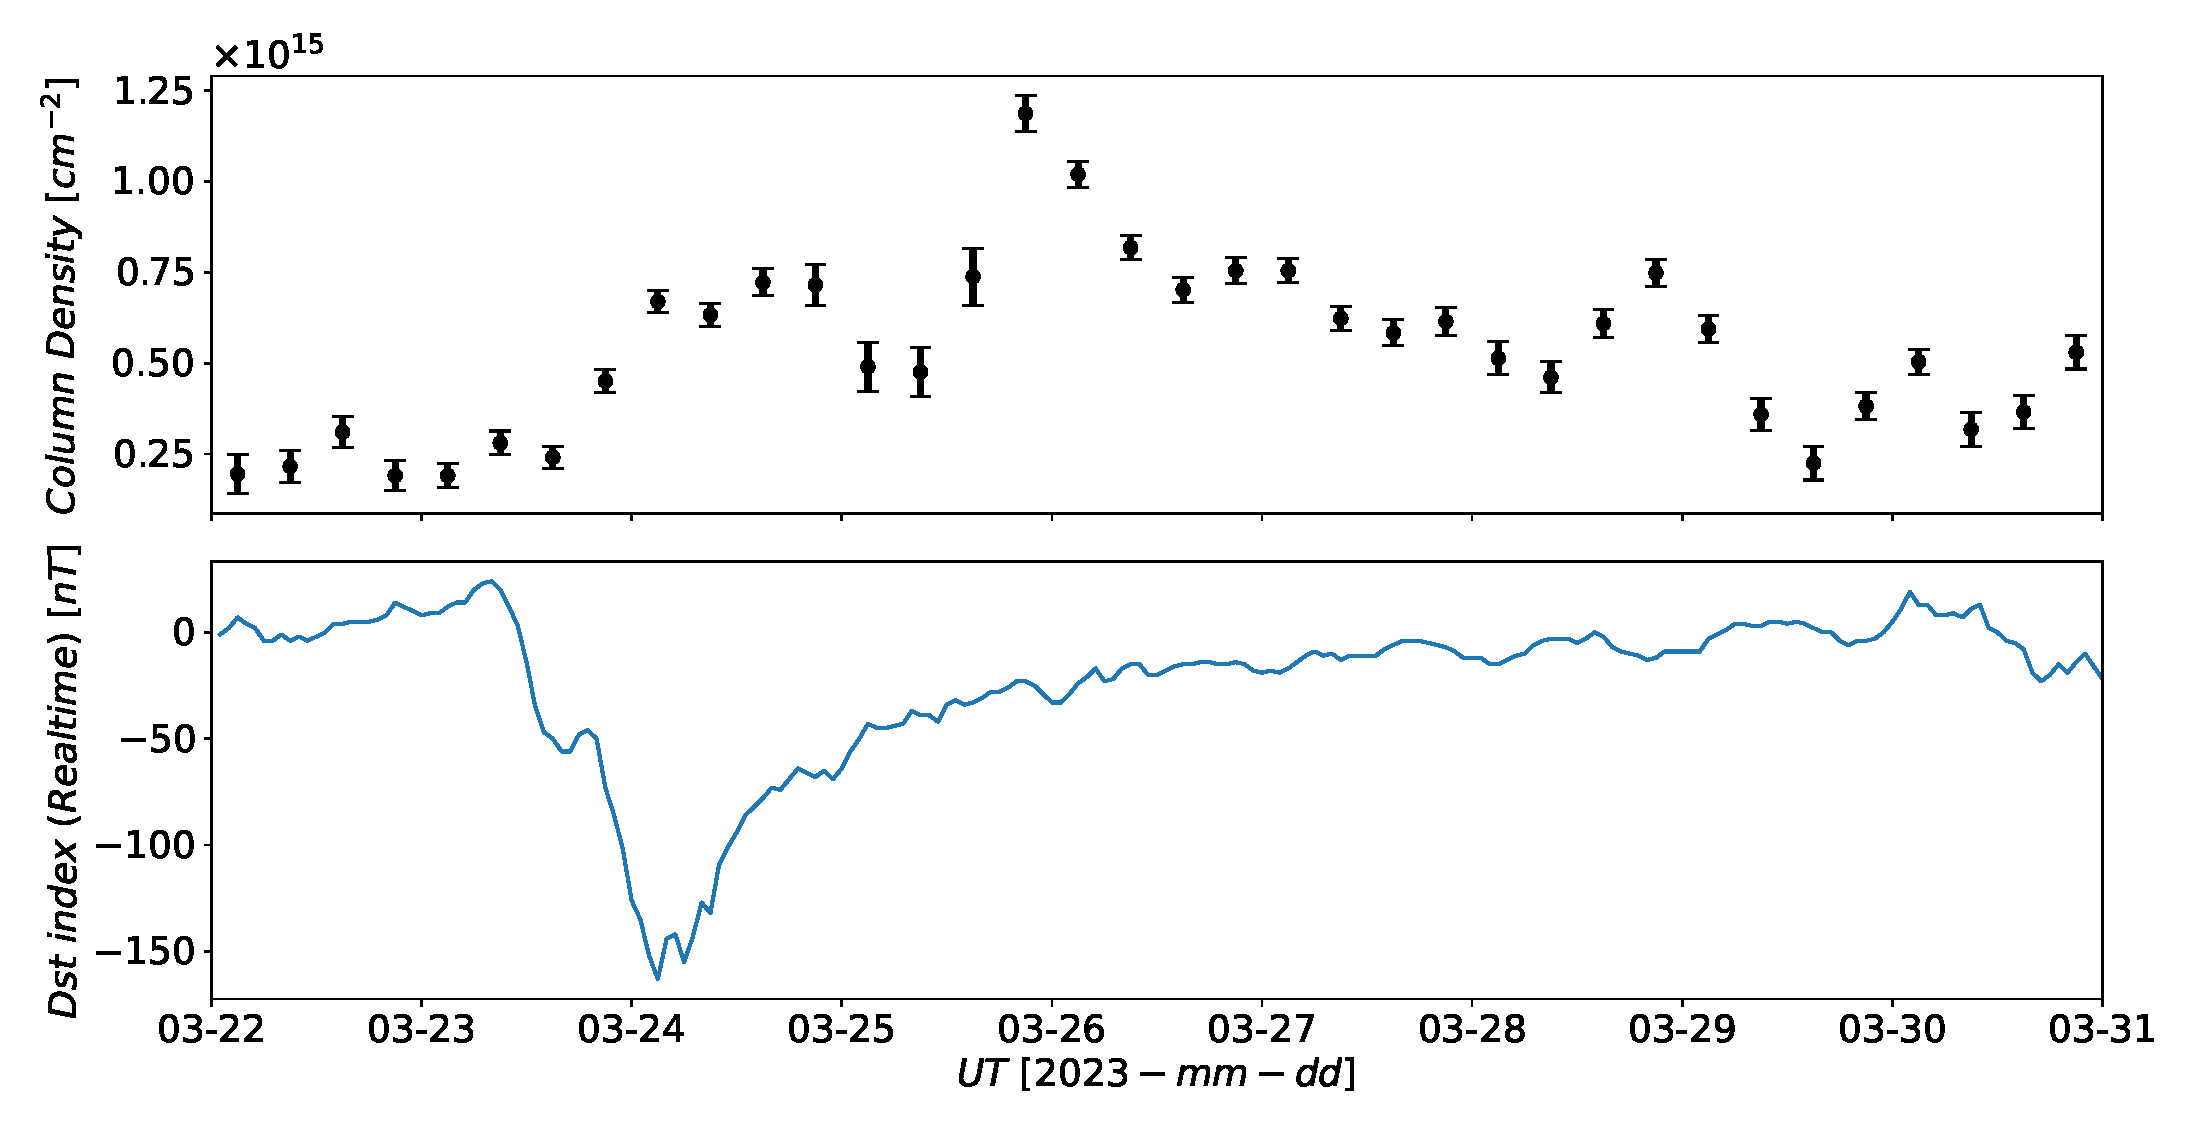
\includegraphics[width=\linewidth]{master_thesis_contents/master_thesis_fig/column_density_spectr6_dst_syowa.pdf}
    \caption{昭和基地における柱密度(1段目。図\ref{fig:column_density_spectr6_syowa}と同様)とDst指数 速報値(2段目)との比較}
    \label{fig:dst_mmcd_syowa}
\end{figure}
\ce{NO}の柱密度の増加が確認できた時期に対応してDst指数の急激な減少がみられた。
とくに、トロムソにおいては急激な\ce{NO}の柱密度の増加があった2019年2月1日〜2019年2月4日、昭和基地においては2023年3月24日の未明前後における\ce{NO}の柱密度の増加に対応して、Dst指数の急激な減少が確認できた。
また、比較的小規模ではあるが、トロムソにおいては2019年1月23日〜2019年1月27日においても、Dst指数の減少が確認された。
この結果より地磁気擾乱によって加速された電子により\ce{NO}が増加した可能性が考えられる。
しかし、それ以外で\ce{NO}の柱密度の増加が確認できた時期において、Dst指数の急激な減少は確認できなかった期間があった。


\subsection{POES/MetOp衛星の電子フラックスデータとの比較}
\label{ssec:comparison_poes}
次に、実際にEEPがどの程度あったのか調べるため、POES/MetOp衛星の電子フラックスデータを用いた比較を行った。
観測場所周辺に降り込む電子のフラックスデータを調べるため、用いるデータの絞り込みを行った(詳細は付録\ref{app:poes})。
トロムソと昭和基地における比較結果をそれぞれ図\ref{fig:poes_mmcd_tromsoe}、図\ref{fig:poes_mmcd_syowa}に示す。
電子フラックスデータは電子がもつエネルギーについて、4つの範囲($>40\ \mathrm{keV}$, $>130\ \mathrm{keV}$, $>287\ \mathrm{keV}$, $>612\ \mathrm{keV}$)に分けて表してある。
\begin{figure}[htbp]
    \centering
    \begin{minipage}{\linewidth}
        \centering
        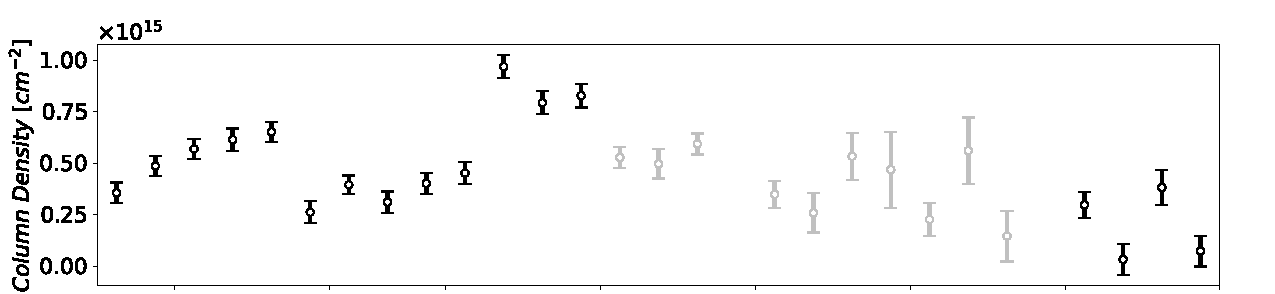
\includegraphics[width=\linewidth]{master_thesis_contents/master_thesis_fig/avg_ColumnDensity_tromsoe_trim.pdf}
    \end{minipage}
    \begin{minipage}{\linewidth}
        \centering
        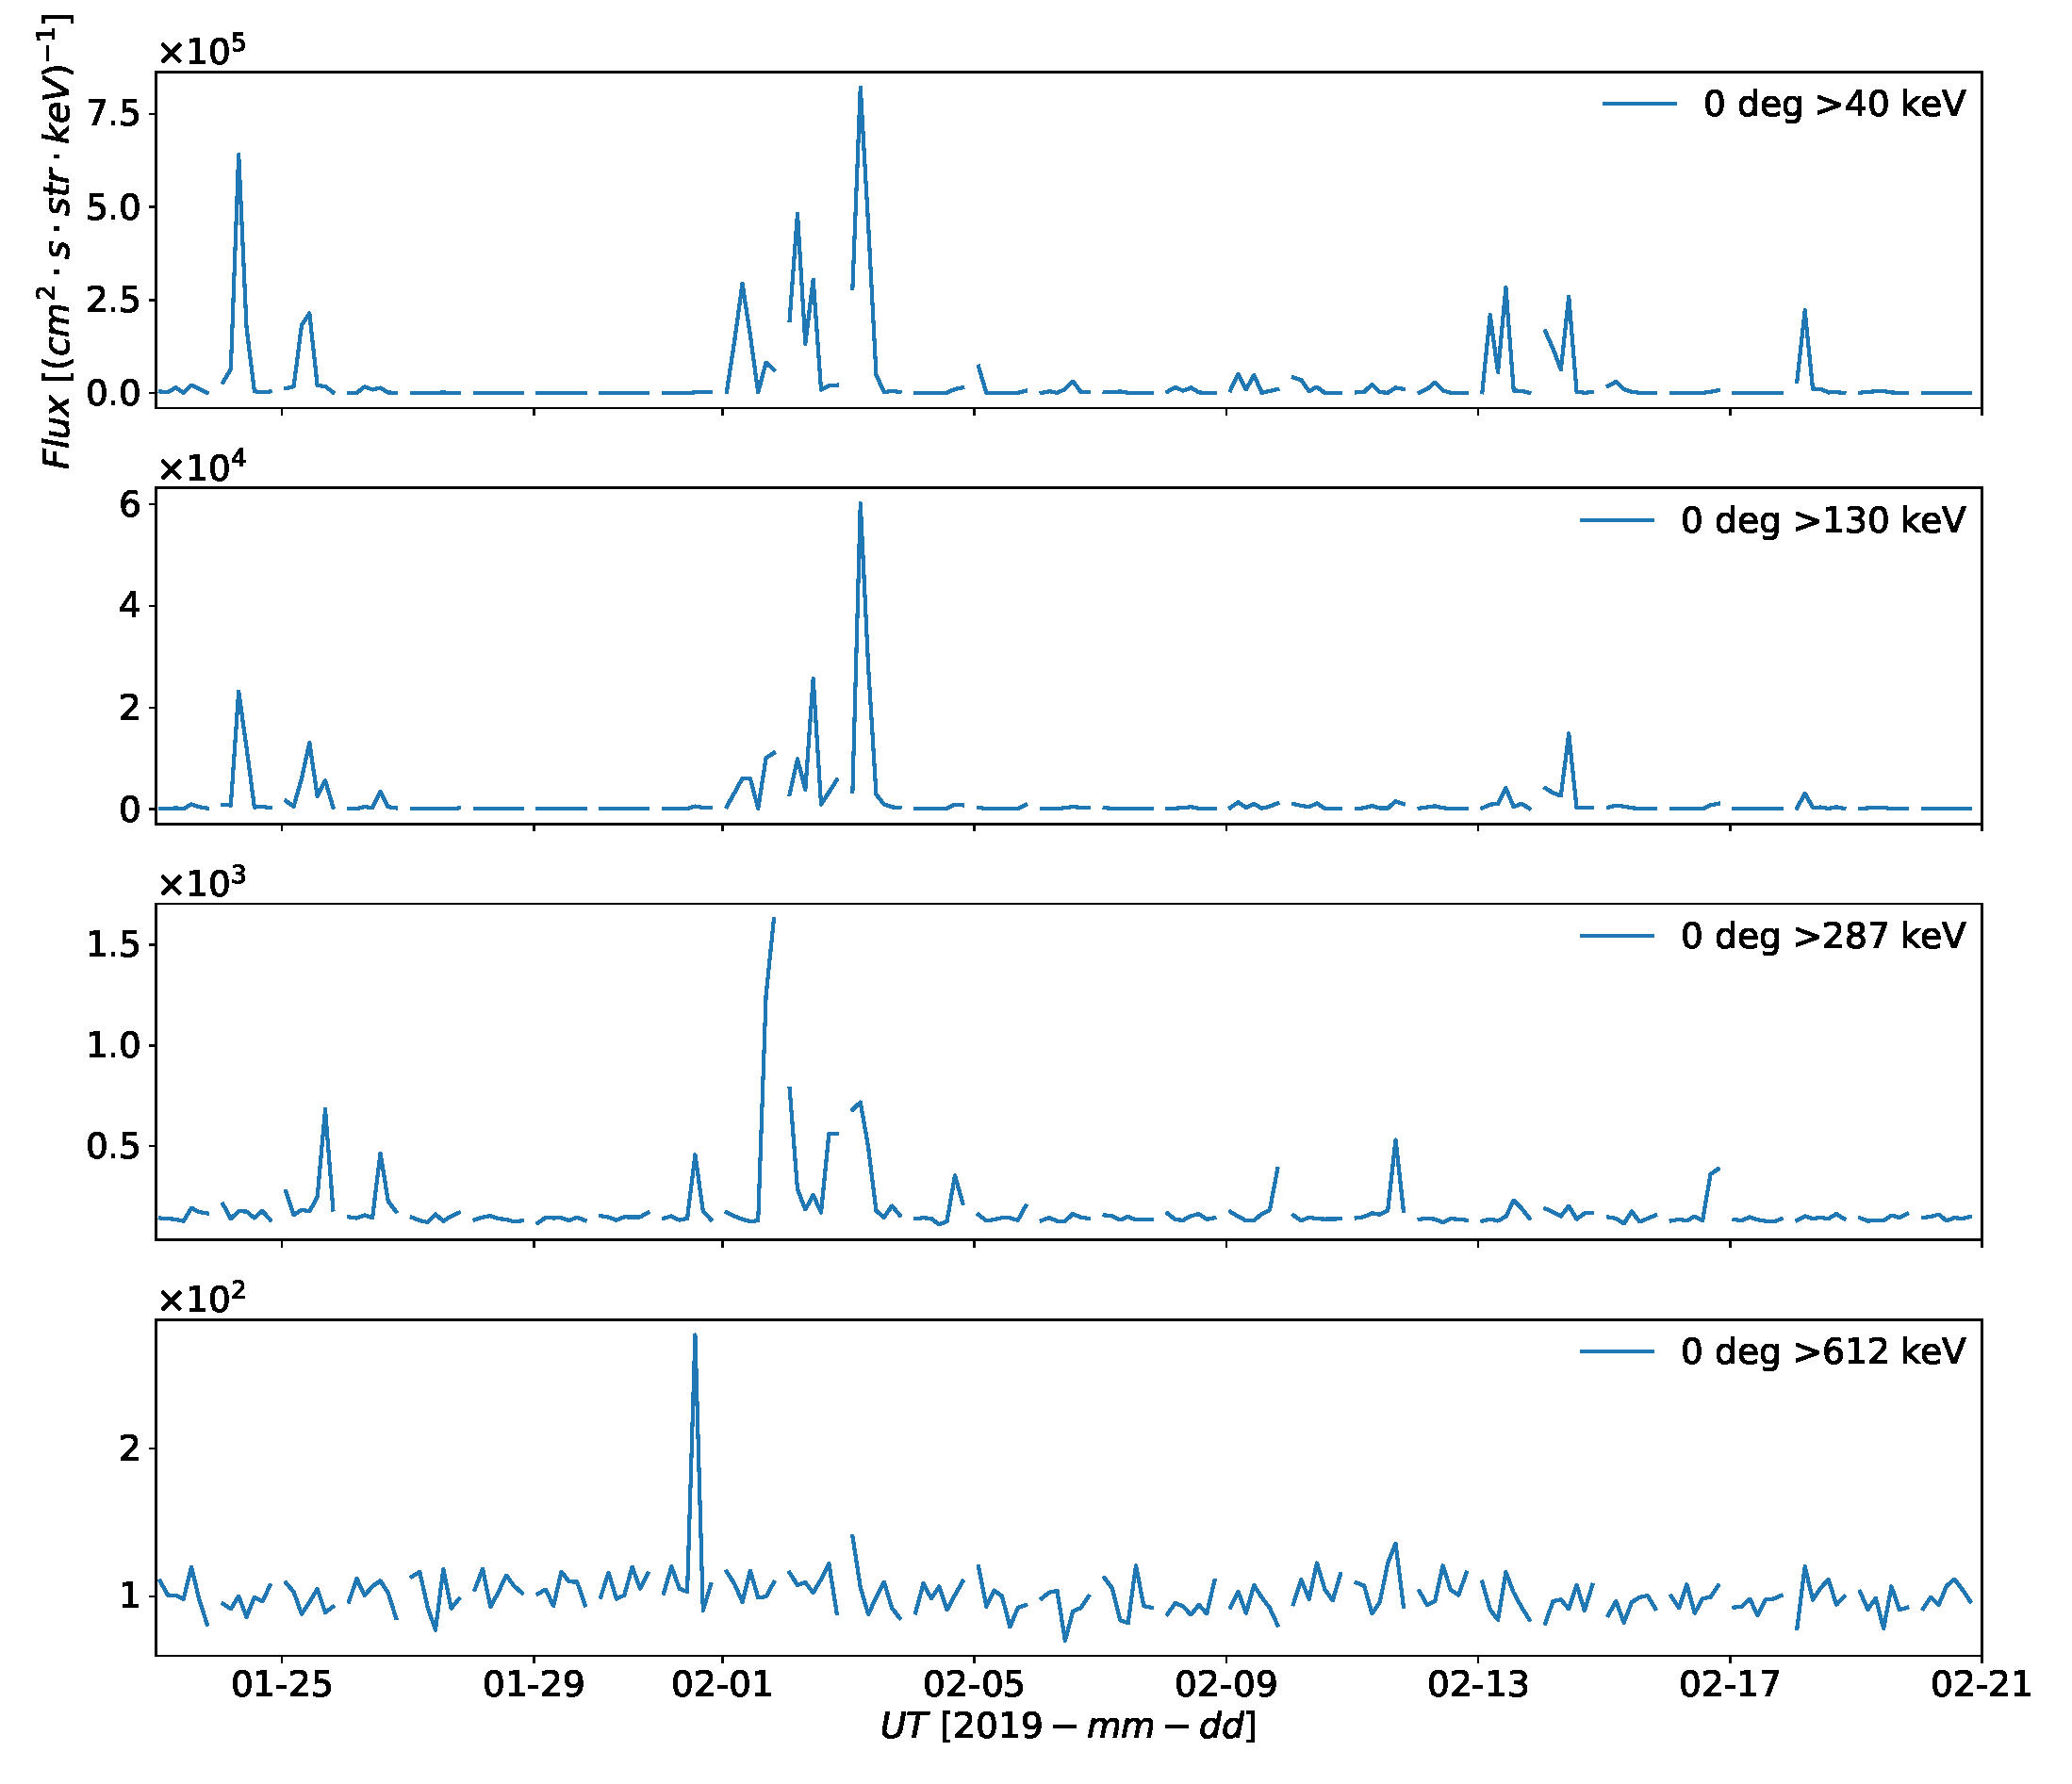
\includegraphics[width=\linewidth]{master_thesis_contents/master_thesis_fig/poes_tromsoe_0deg.pdf}
    \end{minipage}
    \caption{トロムソにおける柱密度(1段目。図\ref{fig:avg_ColumnDensity_tromsoe}と同様)と電子フラックスデータ(2-5段目)との比較}
    \label{fig:poes_mmcd_tromsoe}
\end{figure}
\begin{figure}[htbp]
    \centering
    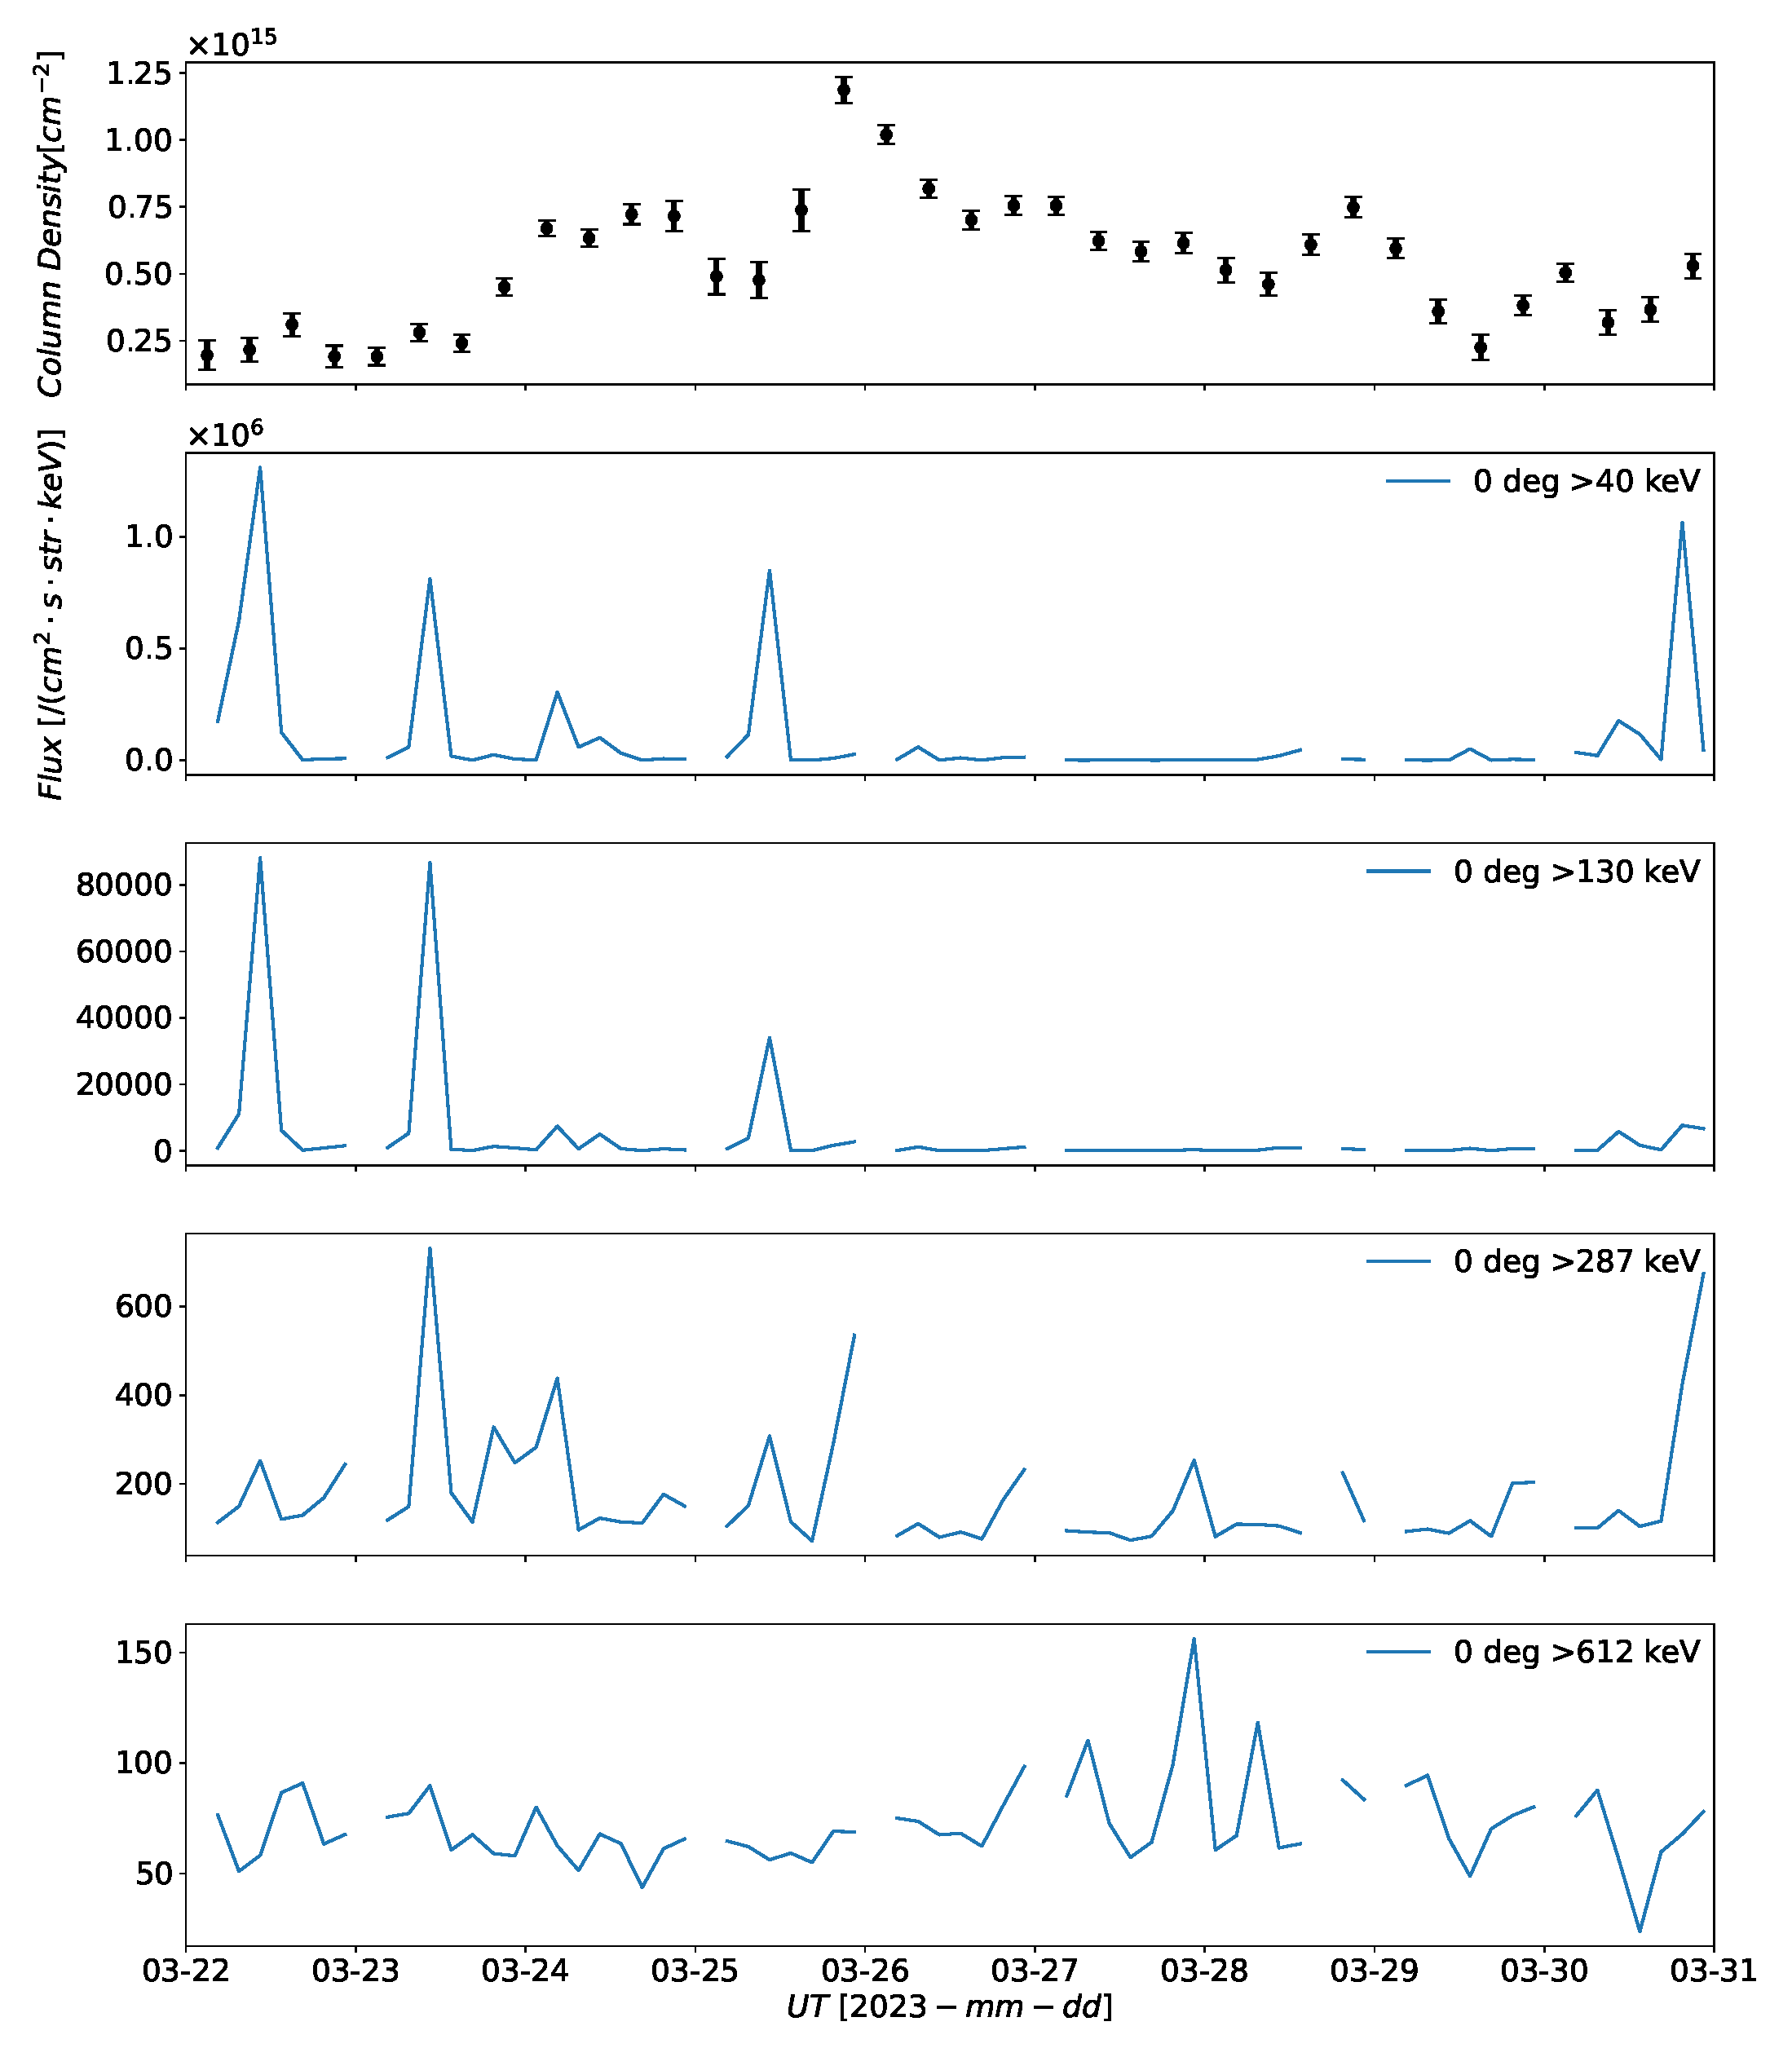
\includegraphics[width=\linewidth]{master_thesis_contents/master_thesis_fig/column_density_spectr6_poes0deg_syowa.pdf}
    \caption{昭和基地における柱密度(1段目。図\ref{fig:column_density_spectr6_syowa}と同様)と電子フラックスデータ(2-5段目)との比較}
    \label{fig:poes_mmcd_syowa}
\end{figure} \par

トロムソと昭和基地どちらにおいても、柱密度の増加に対応して電子フラックスの増加がみられた。
ただし、おおまかな対応関係があることは確認できたが、1対1で対応できるほど相関はよくなかった。\par

トロムソにおいては、Dst指数の急激な減少が確認でき、急激な\ce{NO}の柱密度の増加があった時期(2019年2月1日〜2019年2月4日)は電子フラックスの値も比較的大きく、$>287\ \mathrm{keV}$, $>612\ \mathrm{keV}$などのエネルギーが大きい電子フラックスにおいても値の上昇が確認できた。
また、Dst指数が比較的小さな減少があり、\ce{NO}の柱密度の緩やかな増加があった時期(2019年1月23日〜2019年1月27日)についてはどのエネルギーの範囲の電子フラックスの値も2019年2月1日〜2019年2月4日と比べると小さいことが分かった。\par

昭和基地においても、Dst指数の急激な減少が確認でき、\ce{NO}の柱密度の増加があった時期(2023年3月23日21時〜2023年3月24日3時)は電子フラックスの増加が確認された。
Dst指数の急激な減少が確認できなかったものの、\ce{NO}の柱密度の増加があった時期(2023年3月25日9時〜2023年3月25日21時)においても電子フラックスの増加が確認された。
しかし、柱密度の増加が確認できなかった期間において、比較的小さいエネルギー($>40\ \mathrm{keV}$, $>130\ \mathrm{keV}$)における電子フラックスの増加がみられた。
これは、電子が\ce{NO}が存在する高度まで到達するのに十分なエネルギーをもっていないため、\ce{NO}の増加があまり顕著でない可能性が考えられる。
\par

以上より、磁気嵐以外にも他の要因でEEPの規模に影響を与えると考えられ、\ce{NO}の増加のしかたにも影響を与えている可能性がある。
その要因を探るため、最後にOMNI Data Setを用いた比較を行った。


\subsection{OMNI Data Setとの比較}
\label{ssec:comparison_omni}
柱密度の増加に寄与しない電子フラックスの増加の要因を探るため、磁気圏と電離層の様子を調べることができるOMNI Data Set\footnote{\url{https://omniweb.gsfc.nasa.gov/form/omni_min.html}}を用いた比較を行った(OMNI Data Setの詳細は付録\ref{app:omni})。
トロムソと昭和基地における比較結果をそれぞれ図\ref{fig:omni_mmcd_tromsoe}、図\ref{fig:omni_mmcd_syowa}に示す。
ここで、SYM/HはDst指数の1分値に相当するものであり、AE指数はサブストームに伴う電流の大きさを表すものである~\cite{wdc2009asysym,wdc2022onAEindex}。
昭和基地の解析した期間についてはAE指数は\today 時点で公開されていないため、昭和基地における柱密度との比較ではAE指数は用いていない。\par
\begin{figure}[htbp]
    \centering
    \begin{minipage}{\linewidth}
        \centering
        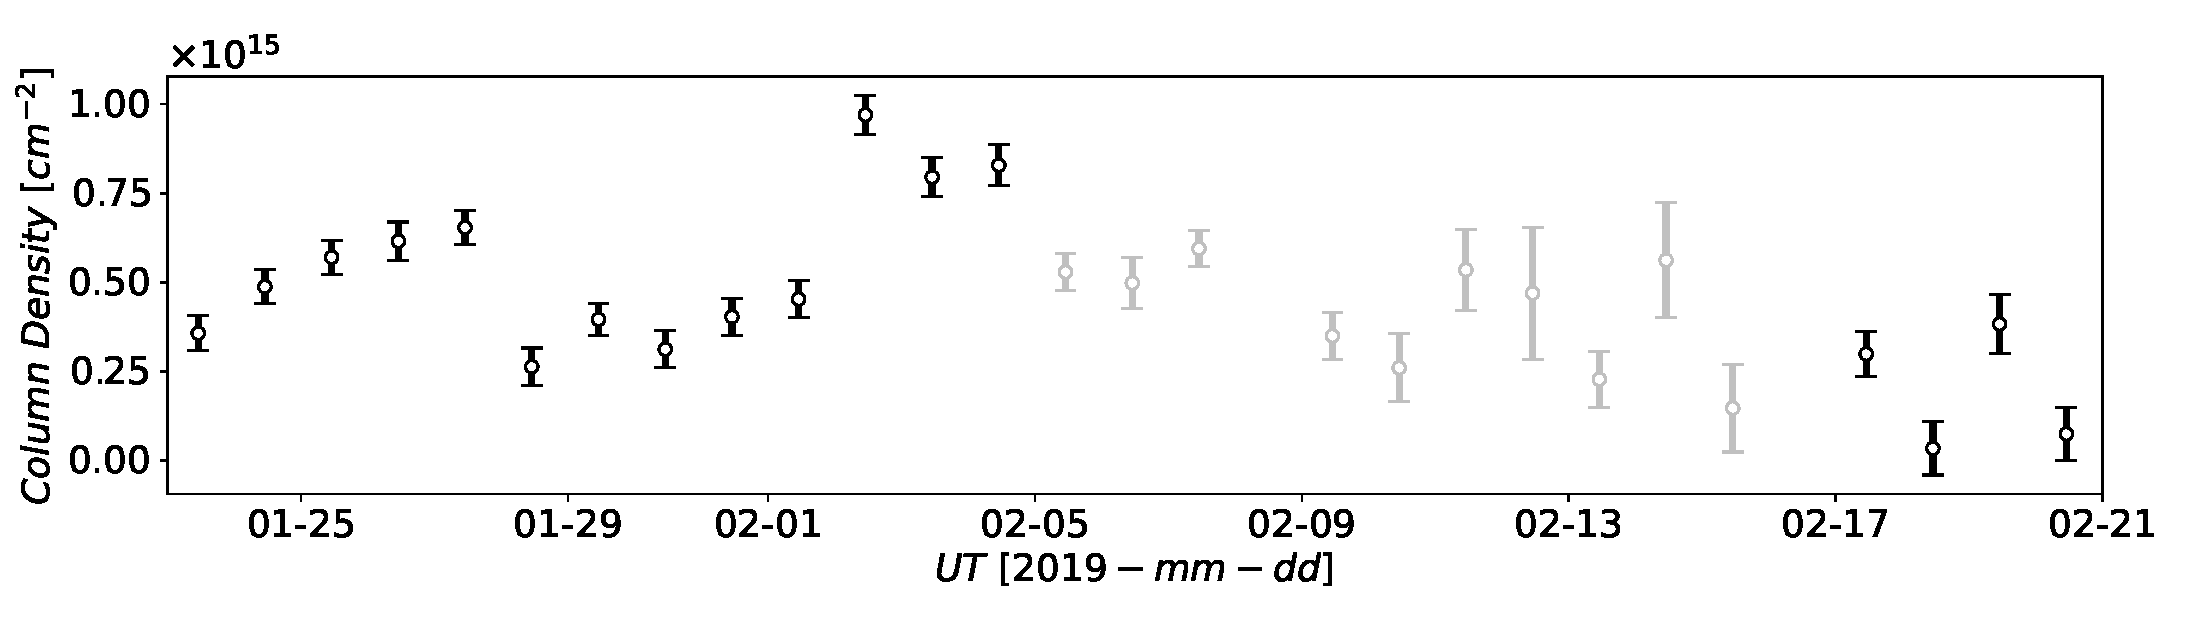
\includegraphics[width=\linewidth]{master_thesis_contents/master_thesis_fig/avg_ColumnDensity_tromsoe.pdf}
    \end{minipage}
    \begin{minipage}{\linewidth}
        \centering
        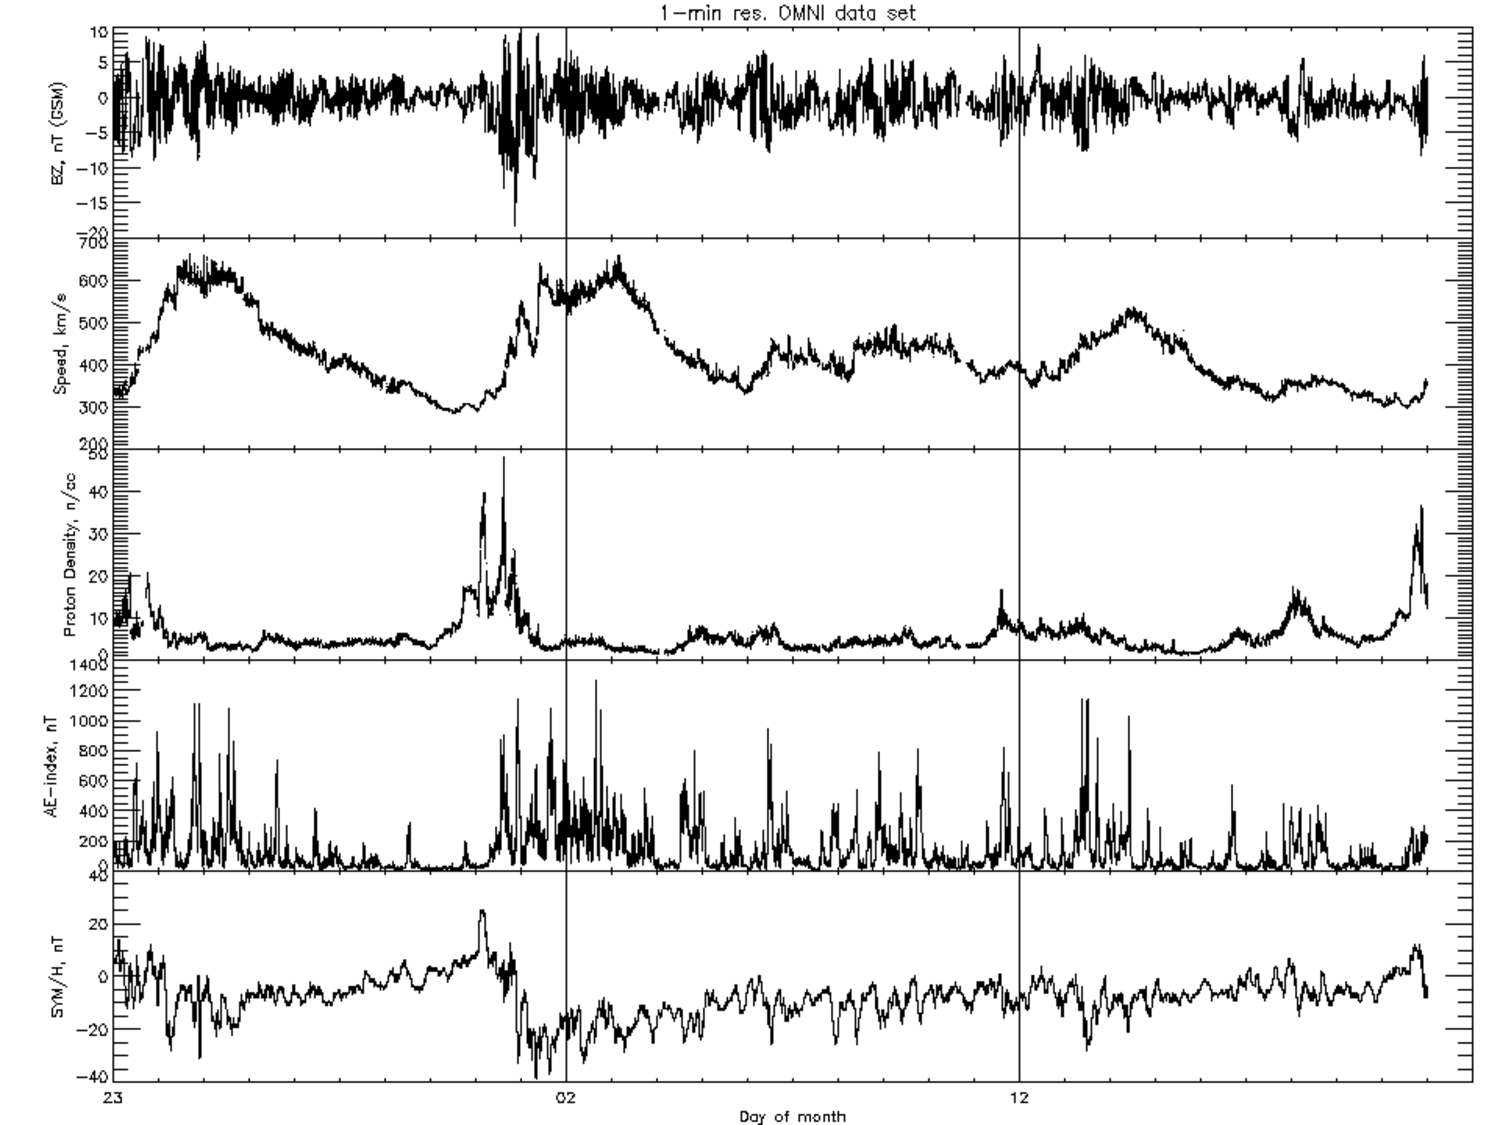
\includegraphics[width=\linewidth]{master_thesis_contents/master_thesis_fig/omni_tromsoe.pdf}
    \end{minipage}
    \caption{トロムソにおける柱密度(1段目。図\ref{fig:avg_ColumnDensity_tromsoe}と同様)とOMNI Data Set(2段目:地球磁場の南北成分、3段目:太陽風の速さ、4段目:プロトン密度、5段目:AE指数、6段目:SYM/H)との比較}
    \label{fig:omni_mmcd_tromsoe}
\end{figure}

トロムソにおいては、柱密度の増加が確認された2つの時期(2019年1月23日〜2019年1月27日と2019年2月1日〜2019年2月4日)どちらにおいても、地球磁場の南北成分のゆらぎが確認できた。
また、太陽風の速さも大きくなっており、AE指数も何度も激しく値が上昇している。
以上より、SYM/H(もしくは図\ref{fig:dst_mmcd_tromsoe}のDst指数)の値をみると磁気嵐としての規模に違いはあるが、対象の時期では高速太陽風が吹いており、サブストームが活発にあったことが考えられる。
2019年2月1日〜2019年2月4日の時期においては、プロトンの密度も上昇していることが確認された。\par
\begin{figure}[htbp]
    \centering
    \begin{minipage}{\linewidth}
        \centering
        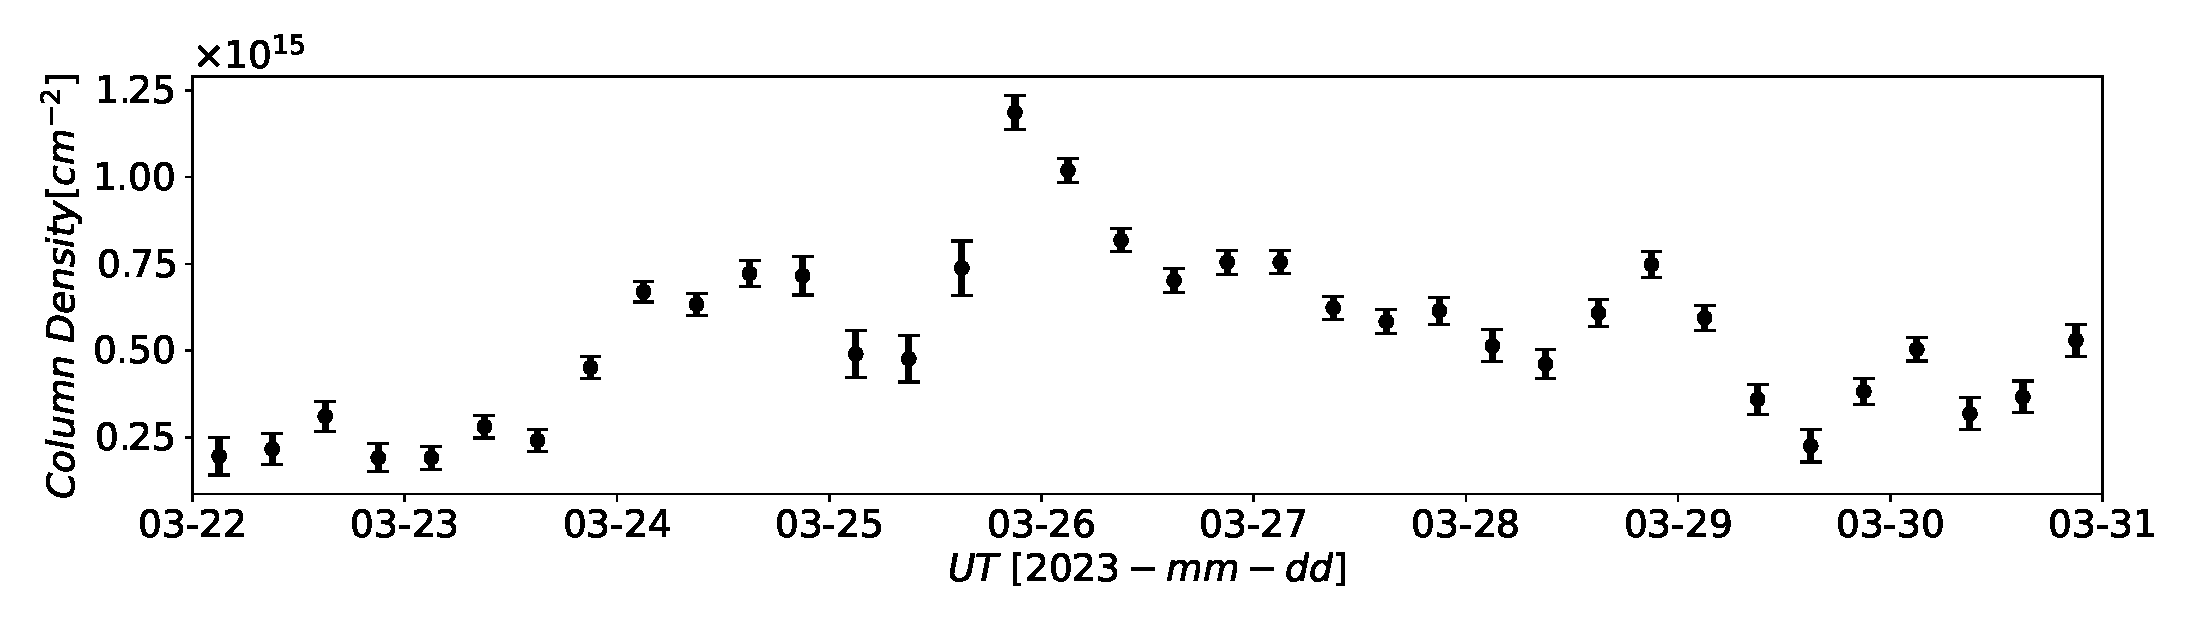
\includegraphics[width=\linewidth]{master_thesis_contents/master_thesis_fig/column_density_spectr6_syowa.pdf}
    \end{minipage}
    \begin{minipage}{0.96\linewidth}
        \centering
        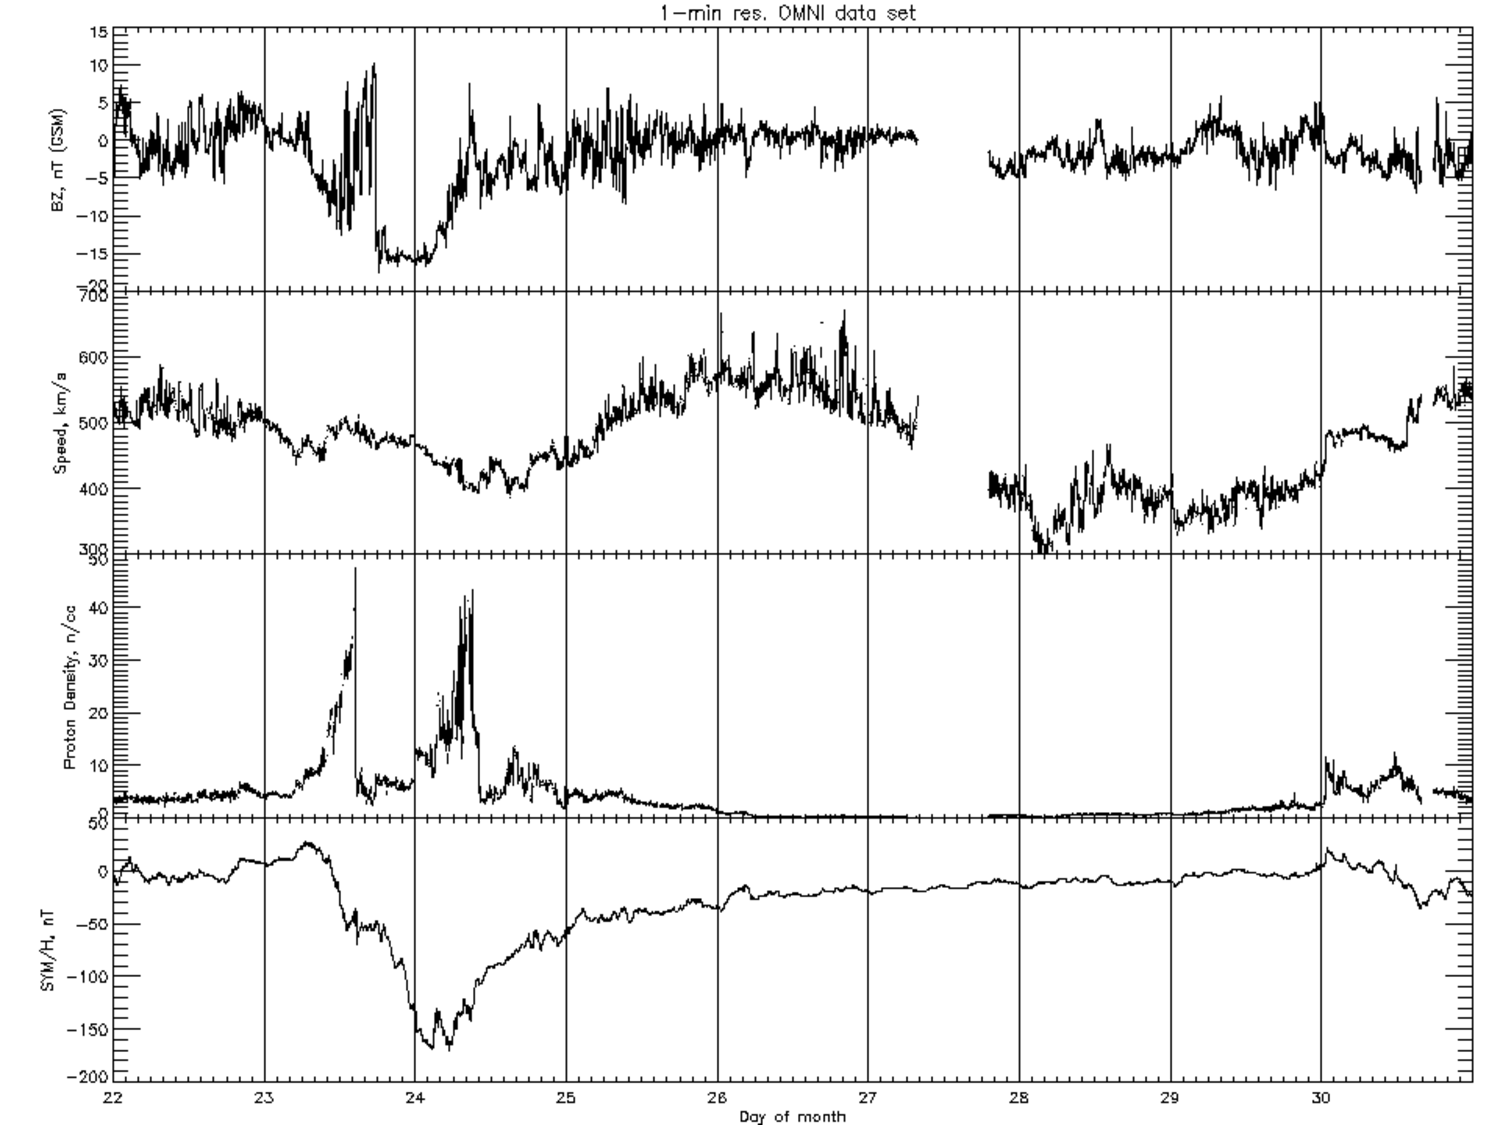
\includegraphics[width=\linewidth]{master_thesis_contents/master_thesis_fig/omni_syowa.pdf}
    \end{minipage}
    \caption{昭和基地における柱密度(1段目。図\ref{fig:avg_ColumnDensity_tromsoe}と同様)とOMNI Data Set(2段目:地球磁場の南北成分、3段目:太陽風の速さ、4段目:プロトン密度、5段目:SYM/H)との比較}
    \label{fig:omni_mmcd_syowa}
\end{figure}

昭和基地においては、磁気嵐の発生と対応して柱密度が増加した2023年3月23日〜2023年3月24日において地球磁場が南方向を向いており、プロトンの密度も上昇していることが確認された。
しかし、高速太陽風は確認できなかった。
もう1つ柱密度の増加が確認できた2023年3月25日においては、SYM/H(もしくは図\ref{fig:dst_mmcd_syowa}のDst指数)の値をみると磁気嵐は回復相にあたるが、高速太陽風があることが確認できた。
これは高速太陽風の影響で電子が加速され\ce{NO}の増加につながった可能性が考えられる。
